%\documentclass{frontiersENG} % for Engineering articles
\documentclass{frontiersSCNS} % for Science articles
%\documentclass{frontiersMED} % for Medicine articles
%\documentclass{frontiersFPHY} % for Physics articles


%\usepackage[utf8x]{inputenc}
%\usepackage[T1]{fontenc}

%\usepackage[english]{babel}

\usepackage{graphicx}
\graphicspath{{figs/}}
\usepackage{tikz}
\usetikzlibrary{shapes}
%
\usepackage{amsmath} 
\usepackage{mathptmx}      % use Times fonts if available on your TeX system
%
\usepackage{color, soul}
\usepackage{url}
\usepackage{multirow}
\usepackage{array}
\usepackage{fixltx2e}
\usepackage{textcomp}

\usepackage[bookmarks]{hyperref}

\usepackage[draft, nomargin, marginclue, footnote]{fixme}
\fxsetup{targetlayout=color}

\newcommand{\eg}{{\textit{e.g.~}}}
\newcommand{\etal}{{\textit{et al.~}}}
\newcommand{\ie}{{\textit{i.e.~}}}

\hyphenation{com-mon-ly}

% Leave a blank line between paragraphs in stead of using \\

\copyrightyear{}
\pubyear{}

\def\journal{Cognitive Science}%%% write here for which journal %%%
\def\DOI{}
\def\articleType{Research Article}
\def\keyFont{\fontsize{8}{11}\helveticabold }
\def\firstAuthorLast{Fink {et~al.}} %use et al only if is more than 1 author
\def\Authors{Julia Fink\,$^{*}$, S\'{e}verin Lemaignan\, Claire Braboszcz and Pierre Dillenbourg}
\def\Address{Computer-Human Interaction in Learning and Instruction (CHILI) \\ Ecole Polytechnique F\'{e}d\'{e}rale de Lausanne (EPFL) \\ CH-1015 Lausanne, Switzerland}
\def\corrAuthor{Julia Fink \vspace{1mm}}
\def\corrAddress{EPFL - CHILI, RLC D1 740, Station 20, CH-1015 Lausanne, Switzerland}
\def\corrEmail{julia.fink@epfl.ch}


\begin{document}
\onecolumn
\firstpage{1}

\title[Dynamics of Anthropomorphism]{Dynamics of Anthropomorphic Effects in Human-Robot Interaction}
\author[\firstAuthorLast ]{\Authors}
\address{}
\correspondance{}
\extraAuth{}
\topic{The Uncanny Valley Hypothesis and Beyond}% If your article is part of a Research Topic, please indicate here which.

\maketitle


\abstract{While anthropomorphism in robotics is a commonly discussed trait of
HRI, it paradoxically lacks formal grounds. This article
attempts first at providing a comprehensive synthesis of the social
phenomenon of \textit{perceiving human-like characteristics in non-human
agents and attributing those characteristics to robots}. We draw on
social sciences and psychology, as well as on a critical survey of
existing literature in the HRI community, to ground the concept of
\textit{anthropomorphism}. Supported by extensive literature review
and long-term field studies, we suggest to go beyond the traditional
perception of anthropomorphism as a static feature of a system: we propose to
understand anthropomorphism as a dynamic, non-monotonic and context-dependent
process, which evolves over time and accounts for special events such as the
so-called \textit{novelty effect}. To this end, we introduce a model of
anthropomorphism that analyzes the phenomenon along three interaction phases,
and we discuss cognitive interpretations that follow.
}


%\keywords{Anthropomorphism, Design, Human-Robot Interaction, Social Issues in Robotics, Acceptance of Robots}


%%%%%%%%%%%%%%%%%%%%%%%%%%%%%%%%%%%%%%%%%%%%%%%%%%%%%%%%%%%%%%%%%%%%%%%%%
%
%
%
%		INTRODUCTION & OVERVIEW
%
%
%
%%%%%%%%%%%%%%%%%%%%%%%%%%%%%%%%%%%%%%%%%%%%%%%%%%%%%%%%%%%%%%%%%%%%%%%%%

% JULIA: brief problem definition / issue, motivation, objectives, contribution ...

\vspace{2cm}
\section{Introduction and Overview}
\label{sec:intro}

%DEFINITION OF ANTHROPOMORPHISM

The essence of anthropomorphism is the perception of human-like characteristics
in either real or imagined non-human agents. According to Epley \textit{et al.}
\cite{epley_when_2008}, these human-like characteristics may include physical
appearance, emotional states perceived to be uniquely human, or inner mental
states and motivations. Real or imagined non-human agents can be "anything that
acts -- or is believed to act -- with apparent independence, including non-human
animals, natural forces, religious agents, technological gadgets, or mechanical
devices". Such anthropomorphic representations are important determinants of how
a person perceives and in turn behaves towards these agents, or how a person may
behave in light of these agents \cite{epley_when_2008}.

%ANTHROPOMORPHISM AS SUBJECT IN HCI AND HRI	
	
Phenomenons related to anthropomorphism -- along with questions such as "how
much human do we perceive in the non-human" or "how human-like do we treat
non-human artifacts" (and why?) -- have received remarkable attention in the
domains of Human-Computer Interaction (HCI) and Human-Robot Interaction (HRI):
the study of humans interacting with an artificial system / machine. Following
the \textit{Media Equation}, it has been described that people mindlessly react
socially to computers \cite{reeves_media_1996} and may even attribute human
(social) characteristics to their artificial counterpart. The phenomenon has
also been observed with virtual characters \hl{cite [50, 100] in rosenthal-von
der P{\"u}tten (2013)}, and more recent studies investigated how far people
ascribe personality or intentions to artificial embodied agents or whether they
show empathetic behavior toward robots
\cite{rosenthal-vonderputten_experimental_2013}. The common base for this
research is the assumption that humans perceive or react to a non-human agent or
artifact as somewhat similar to a human.

In this article we will use the term \emph{anthropomorphic effect} to denote
observable correlates of anthropomorphism. With these we include, amongst
others, verbal utterances (such as direct speech or the use of pronouns
"he/she"), (social) gestures (such as a hug, waving, deictic gestures) or
\hl{anticipation of certain actions of an agent [what??]}.

%CONTROVERSAL UNDERSTANDINGS OF ANTHROPOMORPHISM

However, not everything colloquially labeled as \emph{anthropomorphism} really
is anthropomorphism. Different, even partially conflicting, understandings of
anthropomorphism exist across and within disciplines
\cite{duffy_anthropomorphism_2002}. Epley \textit{et al.} \cite{epley_when_2008}
try to narrow down and clarify the understanding of anthropomorphism in
psychology by explaining what it is \textit{not}. The authors list four things
that anthropomorphism does not include: First, anthropomorphism does not include
behavioral descriptions of observable actions. Anthropomorphism requires going
beyond what is directly observable. Second, anthropomorphism does not merely
entail animism, as animate life is not a uniquely human-like characteristic.
Third, anthropomorphism does not include any requirement of reasoned or
reflective endorsement of an inference (\hl{the strength of anthropomorphic
inferences can vary} \footnote{for further explanation the reader may refer to
the original work \cite{epley_when_2008}.}).	Finally, anthropomorphism is not
necessarily inaccurate. A psychological theory should take this (in)accuracy in
anthropomorphism into account and predict variability in the tendency to
perceive human-like traits in non-human agents.  In conclusion, it has been
noted that anthropomorphism is a very complex phenomenon - in itself, its
understanding, and when studying it. A common formal ground is missing; however,
it is important to be clear about what exactly we mean when using the term
anthropomorphism.


%%%%%%%%%%%%%%%%%%%%%%%%%%%%%%%%%%%%%%%%%%%%%%%%%%%%%%%%%%%%%%%%%%%%%%%%%
%
%
%
%		PART 1: WHAT OTHERS DID AND WE ALREADY KNOW ABOUT ANTHROPOMORPHISM
%
%
%
%%%%%%%%%%%%%%%%%%%%%%%%%%%%%%%%%%%%%%%%%%%%%%%%%%%%%%%%%%%%%%%%%%%%%%%%%
%
% JULIA: there will be 4-5 subsections
%	1) anthropomorphism as a social phenomenon, definitions, origins, etc.
%	2) anthropomorphism as a consequence of anthropomorphic / life-like design
%	3) the link to robotics and HRI, mention the uncanny valley theory ...
%	4) however: we suggest anthropomorphism is more than a static feature ...
%
%

\vspace{2cm}
\section{Anthropomorphism}
\label{sec:anthropomorphism}

\hl{bridge sentence}



\subsection*{Anthropomorphism as a Social Phenomenon}
\label{sec:social-phenomenon}

The term \textbf{anthropomorphism} is used in different senses throughout
natural sciences, psychology, Human-Computer Interaction, and Human-Robot
Interaction \cite{duffy_anthropomorphism_2003}. Originally, anthropomorphism
comes from the Greek \textit{`anthropos'} for `man' (or `human') and
\textit{`morphe'} for `form/structure' (or `shape'). It can be understood as
people's tendency to think of objects as if they had human characteristics, and
consequently, attribute / ascribe specific human characteristics to these
non-human entities and artifacts (including animals, and robots)
\cite{duffy_anthropomorphism_2003,schmitz_concepts_2011}. Apart from
anthropomorphism there is also \textbf{animism}, the \textit{"attribution of
life to the nonliving"} \hl{in Schmitz 2011, cite Piaget original text!}. Often
synonymously used to animism is \textbf{zoomorphism}, which describes the case
when non-lifelike objects are associated with animalistic attributes, excluding
human-specific traits. Both anthropomorphism and zoomorphism can be embraced by
the concept of \textbf{life-likeness}. \footnote{The inverse process would be
called dehumanization \cite{haslam_dehumanization:_2006}, or mechanomorphism
\cite{caporael_anthropomorphism_1986}.}
		
Commonly, anthropomorphism can also be understood as \textbf{humanization} or
\textbf{personification} of anything other than a human being. The phenomenon of
personifying something has ancient roots, \textit{e.g.} in mythology but also in
storytelling. In prehistoric artworks and illustrations, zoomorphic
(animal-shaped) or anthropomorphic shapes were already used to represent natural
forces or great spirits, for instance. A more recent example is Milo Winter's
illustration from 1919, \textit{"The North Wind and the Sun"} (Figure
\ref{fig:1}), in which both north wind and sun are given a human face
(anthropomorphized). Similarly, when parents explain their children about
nature, they tend to use anthropomorphisms, \textit{e.g.} saying the skies would
cry when it rains. More generally, an explanation for why people
anthropomorphize is that by doing so, the subject is made \emph{graspable},
\emph{understandable}, \emph{predictable}, and one feel \emph{more empathetic}
toward it\fxnote{important part. Emphasize this 4 facets, eg by saying we build
on top of them}. For instance, people commonly anthropomorphize their pets,
ascribing mental states, intentions or feelings to them
\cite{eddy_attribution_1993}. Interestingly, pet-ownership seems to have a
significant impact on human-robot interaction: several studies suggest that
pet-owners are more likely to anthropomorphize technologies and robots than non
pet-owners \hl{references!}.

 \begin{figure}\centering
% Use the relevant command to insert your figure file.
% For example, with the graphicx package use
  
\includegraphics[scale=0.91]{north-wind.jpg}
  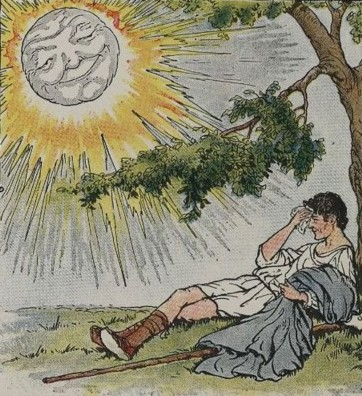
\includegraphics[scale=0.91]{sun.jpg}
% figure caption is below the figure
 \caption{Milo Winter illustration of Aesop Fable \textit{The North Wind and the Sun}, 1919; both natural forces wind and sun are anthropomorphized with a human face; picture source: wikipedia}
 \label{fig:1}       % Give a unique label
 \end{figure}
 

\paragraph{Explanations for Anthropomorphism}
\label{sec:explanations}

\fxfatal{inconsistency: we already give explanations for anthropomorphism in previous paragraph...}

Anthropomorphism represents just one of many examples of induction whereby
``people reason about an unknown stimulus based on a better-known representation
of a related stimulus"~\cite{epley_when_2008}, in this case reasoning about a
non-human agent based on representation of the self or other humans.

According to Lee \etal~\cite{lee_human_2005}, there are two main perspectives in
explaining people's tendency to anthropomorphize. First one explains
anthropomorphism from the design of the artifact. It assumes that humans
directly respond to life-like or social cues that an object or system emits,
without thoughtful mental processing, by simply applying stereotypes and
heuristics to it. In fact, from early childhood on, humans are inherently
well-trained to perceive life \cite{epley_seeing_2007}. Schmitz
\cite{schmitz_concepts_2011} describes that within the visual scope of design,
the outer appearance can have an important impact on the overall perception of
an object. The basic assumption here is that if an artifact appears much like a
human, it is likely to be treated similar to a human. If this explanation of
anthropomorphism is correct, people may respond automatically to social cues
emitted by a robot, and apply human-human social schemas and norms to these
interactions.

The second perspective applies a human-centered, cognitive viewpoint where
anthropomorphism is described through people's specific mental model they
construct about how an artifact works the way it does.  We then
anthropomorphize because it allows us to explain things we do not understand in
terms that we do understand, and what we understand best is ourselves as human
beings. This is consistent with the \emph{familiarity
thesis}~\cite{hegel_understanding_2008} which claims that we understand the
world based upon a mental model of the world that we are most familiar with.
Consequently, people tend to thoughtfully develop a mental model of agents in
their environment and make inferences about it based on what is familiar to
them -- humans and human behavior, for instance.  This point of view implicitly
builds on a person's ability to attribute mental states to oneself and others
(\ie the availability of a \emph{theory of mind}~\cite{premack1978does} -- the
link between a tendency to anthropomorphize and the engagement in the
attribution of mental states to other humans has been recently demonstrated at
the brain level in~\cite{cullen2013individual}). A theory of mind for other
agents enables us to attribute intentionality to those agents
\cite{leslie_pretense_1987,admoni_multi-category_2012}. Previous research
examined the validity of the mental model concept with various kinds of robots
\cite{schmitz_concepts_2011,kiesler_mental_2002}. Findings suggest that people
tend to hold richer mental models of anthropomorphic robots in contrast to
mechanic ones \cite{kiesler_mental_2002}.

According to Lee \textit{et al.} \cite{lee_human_2005}, there are two main
perspectives in explaining people's tendency to anthropomorphize. The first
one explains anthropomorphism from the design of the artifact
(anthropomorphic form in the design). It assumes that humans directly
respond to life-like or social cues that an object or system emits, without
thoughtful mental processing, by simply applying stereotypes and heuristics
to it. In fact, from early childhood on, humans are inherently well-trained
to perceive life \cite{epley_seeing_2007}. Schmitz
\cite{schmitz_concepts_2011} describes that within the visual scope of
design, the outer appearance can have an important impact on the overall
perception of an object. The basic assumption here is that if an artifact
appears much like a human, it is likely to be treated similar to a human. If
this explanation of anthropomorphism is correct, people may respond
automatically to social cues emitted by a robot, and apply human-human
social schemas and norms to these interactions.

The second perspective applies a human-centered, cognitive viewpoint where
anthropomorphism is described through people's specific mental model they
construct about how an artifact works the way it does. According to v.
Foerster \hl{ref} \textit{"we anthropomorphize because it allows us to
explain things we do not understand in terms that we do understand, and what
we understand best is ourselves as human beings"}
\cite{hegel_understanding_2008}. This is consistent with the \hl{familiarity
thesis (18)} \cite{hegel_understanding_2008} which claims we understand the
world based upon a mental model of the world that we are most familiar with.
Consequently, people tend to thoughtfully develop a mental model of agents in
their environment and make inferences about it based on what is familiar to
them. This point of view implicitly builds on a person's ability to attribute
mental states to oneself and others, which is called \textit{Theory of
Mind}~\cite{Premack1978}. A theory of  mind for other agents enables us to
attribute intentionality to those agents
\cite{leslie_pretense_1987,admoni_multi-category_2012}. If a system behaves much
like a human being (\eg emits a human voice), people's mental model of the
system's behavior may approach their mental model of humans, though the model
may differ in some important aspects \hl{ref? Schmitz?}. In turn, people's
estimation of a robot's knowledge model and its capabilities affects the way
they relate to it. Previous research examined the validity of the mental model
concept with various kinds of robots
\cite{schmitz_concepts_2011,kiesler_mental_2002}. Findings suggest that people
tend to hold richer mental models about anthropomorphic robots in contrast to
mechanic ones \cite{kiesler_mental_2002}. Later in this article, we may however
come to question this result for longer human-robot interactions, after one
get's acquantained with the robot's behaviour.


\paragraph{Insights from Social and Developmental Psychology}
\label{sec:psychological-factors}

To understand the social phenomenon of anthropomorphism better, it makes sense
to take a look at studies and explanations from developmental psychology. The
phenomenon of attributing intentions and \hl{animacy} to simple shapes based on
motion has been intensively studied in developmental psychology. Two famous
studies on the perception of and attribution to simple things have been done in
the mid 1940s: Heider and Simmel's work on the \textit{attribution theory}
\cite{heider_experimental_1944} and Michotte's studies on \textit{the perception
of causality} \cite{michotte_perception_1963}. In both experiments, participants
viewed animations of simple shapes, such as circles or triangles (see Figure
\ref{fig:animacy_attribution}). Asked to describe what they observed,
interestingly, most people developed elaborate stories, attributing motivations,
emotions and relationships between the objects.

\begin{figure}\centering
% Use the relevant command to insert your figure file.
% For example, with the graphicx package use
  
\includegraphics[scale=0.6]{heider-simmel_animation.jpeg}
% figure caption is below the figure
 \caption{Fritz Heider and Mary-Ann Simmel's animated film to study people's tendency to attribute animacy and intention to simple shapes; \textit{An experimental study of apparent behaviour}, 1944}
 \fxnote{wrap text around this figure?}
 \label{fig:animacy_attribution}       % Give a unique label
 \end{figure}

What is a person's motivation to attribute human characteristics to simple
geometric shapes, or more sophisticated, anthropomorphic shapes, animated or
not? Irrespective of the artifact's characteristics, there are psychological
theories to explain the phenomenon. An interesting recent psychological theory
of anthropomorphism (also related to robotics) is provided by Epley, Waytz, and
Cacioppo \cite{epley_seeing_2007}. The authors established a three-factor theory
of when people are likely to anthropomorphize based on psychological
determinants. Namely, the theory suggests that some people are more likely to
anthropomorphize when:

\begin{itemize}
	\item anthropocentric knowledge is accessible and applicable to the artifact (\textit{elicited agent knowledge}),
	\item they are motivated to explain and understand the behavior of other agents (\textit{effectance motivation}), and
	\item they have the desire for social contact and affiliation (\textit{social motivation}).
\end{itemize}

Epley \textit{et al.} describe that \textit{elicited agent knowledge} is a
\textbf{cognitive determinant  of anthropomorphism} which is understood as the
activation of knowledge about humans (or the self) when making inferences about
non-human agents. One basic reasons for this are a person's physical constraints
of being a human and nothing else. Consequently, one has no other experience
than the self and in turn people tend to make inferences about others' mental
states by relying inordinately on their own mental state. \footnote{Using one's
own mental states and characteristics as a guide when reasoning about other
humans is ego-centrism; when reasoning about non-human agents is
anthropomorphism. See Epley, 2007 \textit{et al.} \cite{epley_seeing_2007}} Also
empirical findings suggest that knowledge about humans in general, or
self-knowledge in particular, is likely to serve as a readily accessible base
for induction when reasoning about non-human agents. This tendency is usually
stronger in young children and decreases with cognitive development and the
learning to distinguish the self from other humans, and non-human agents. 
	
Both \textit{effectance} and \textit{sociality} are \textbf{motivational
determinants of anthropomorphism}. \textit{Effectance} is understood as the
motivation to interact effectively in one's environment: understand, predict,
\hl{reduce uncertainty (this feeds again our hypothesis that as soon as a robot
is not uncertain anymore, there is no need to keep on anthropomorphizing
it)}\fxfatal{important! move/copy that to the 'model' section or discussion}
about one's environment and the agents that inhabit it. According to Epley
\textit{et al.}, anthropomorphism serves as one way to reduce uncertainty and
increase comprehension of events in one's environment. They mention for
instance, children (as they are in their early stages of life) appear to be more
likely to anthropomorphize than adults, as they might feel more uncertain within
their environment.

\textit{Sociality} describes the motivation for social contact, social
connection, and social approval from other agents. Importantly for
anthropomorphism, this social connection appears to be satisfied by connections
with \hl{ \textit{"two of the most commonly anthropomorphized non-human agents,
namely pets and religious agents"}} \cite{epley_seeing_2007}. According to Epley
\textit{et al.}, the motivation of being socially connected increases the
tendency to anthropomorphize non-human agents because first sociality motivation
increases the tendency to perceive human-like characteristics and traits even in
non-human agents, and second it increases the tendency to search for sources of
social connection in one's environment. Consequently, the authors suggest
\textit{"[...] those who are chronically lonely should be more likely to
anthropomorphize nonhuman agents than those who are more chronically
connected"}. 



\subsection*{Anthropomorphic Design Principle}
\label{sec:anthropomorphic-design}

\hl{check if we really need this section ... maybe yes because it is important for the uncanny valley hypothesis}

In general, it is suggested that increasing human-likeness of a robot	 will
lead to more perceived \textit{affinity} from the human side
\cite{mori_uncanny_1970}. This theoretical concept is also supported by
psychological determinants of perceiving human-likeness in something non-human:
\textit{"the more similar in appearance, the more people are likely to use
themselves as a source of induction and anthropomorphize these nonhuman agents"}
\cite{epley_seeing_2007}. Further, empirical studies have shown that robots with
human-like forms can enhance social responses from humans which in turn can have
a positive impact on acceptance
\cite{venkatesh_theoretical_2000,duffy_anthropomorphism_2003,goetz_cooperation_2002}.
People responded more positively to an artifact that displayed human-like
behavioral characteristics (emotions, facial expression) in contrast to a purely
functional design
\cite{eyssel_anthropomorphic_2010,krach_can_2008,reeves_media_1996,riek_how_2009}.
Overall, these results suggest that human-like features in robots enhance
anthropomorphism, and in turn create a social view toward the robot.

Well known from the HRI community, we may mention the other side of human-like
behaviours and appearance: a not yet very well defined thin line separates
acceptable human-like forms in robots from creepy artificial \textit{almost}
human-like appearing robots. The underlying theory for this viewpoint is stated
as the \textit{Uncanny Valley} \cite{mori_uncanny_1970} which suggests that
artificial human-like forms are only acceptable up to a certain degree but lead
to reluctance if they fail in trying to attain human-likeness \hl{cross-ref to
later and figure}.

The theory (Figure~\ref{fig:uncanny_valley}) hypothesizes that a person's
response to a human-like robot would abruptly shift from empathy to revulsion as
it approached, but failed to attain, a lifelike appearance
\cite{mori_uncanny_1970}. Starting with low degrees of anthropomorphic cues in a
robot, humans seem to readily accept and prefer them compared to purely
mechanical robots. In general, one can say that up to a certain (yet not very
well defined) degree, the more human-like the robot, the more affection it can
engender through familiar communication references.


\begin{figure}\centering
% Use the relevant command to insert your figure file.
% For example, with the graphicx package use
  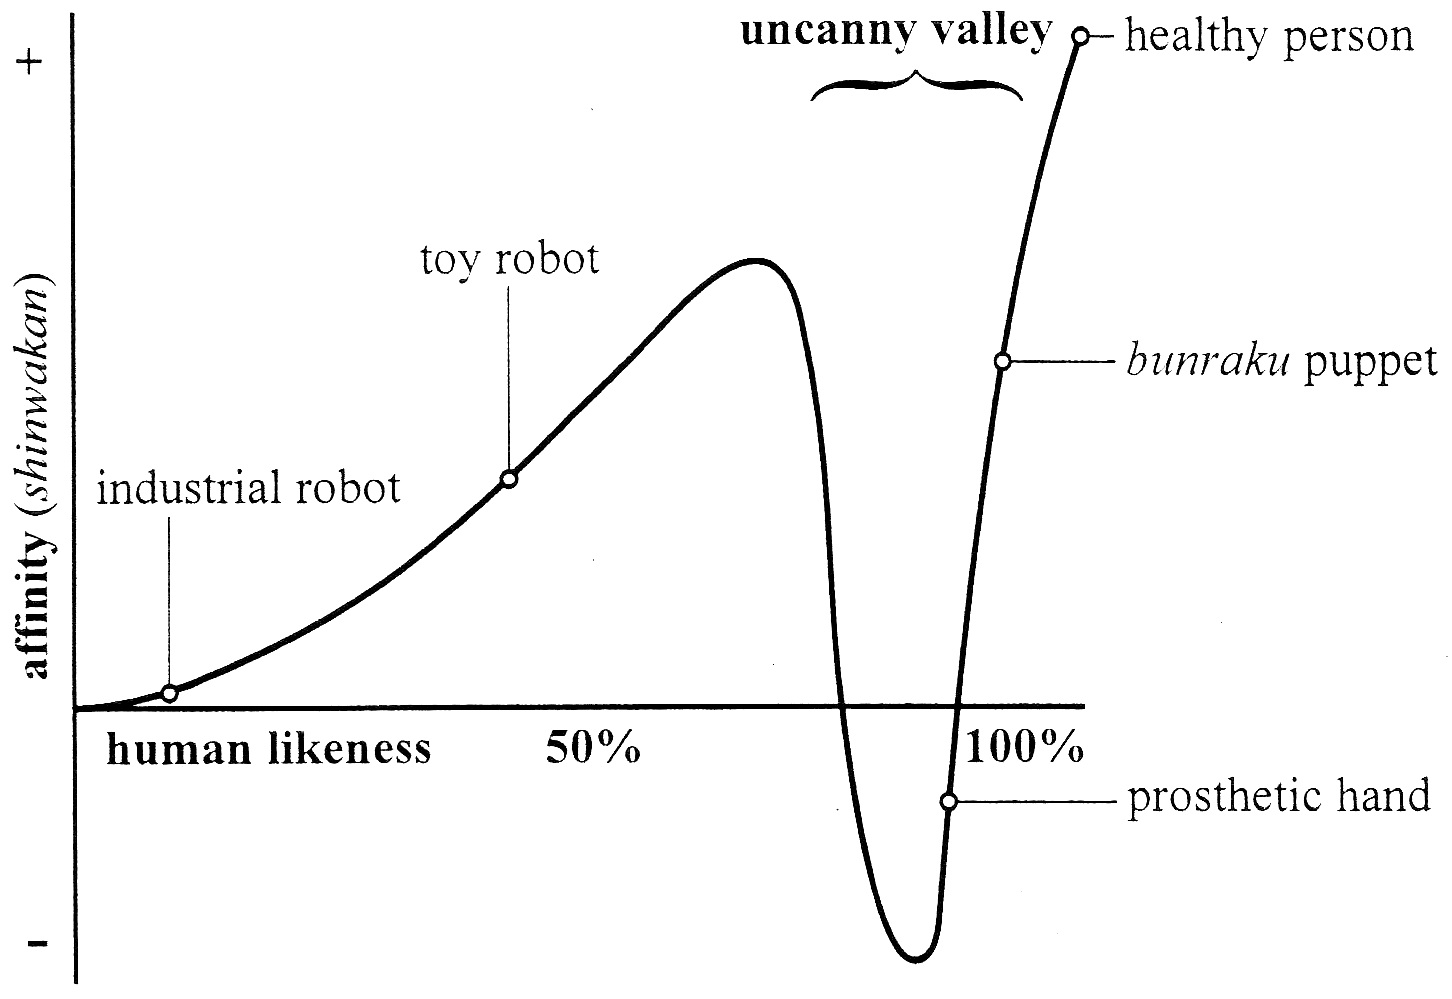
\includegraphics[scale=0.6]{uncanny-valley.jpg}
% figure caption is below the figure
 \caption{Mashiro Mori, illustration of the \textit{Uncanny Valley}, originally
 from 1970; picture from a manuscript version of \cite{mori_uncanny_2012}}

 \label{fig:uncanny_valley}       % Give a unique label
 \end{figure}

Another sensitive aspect is that with robots that closely resemble humans,
ethical issues arise. For instance, we need to consider how far we actually want
an \textit{artificial agent} to resemble ourselves and how far it should act
`artificially socially' toward humans, and what happens as soon as it is
considered a \textit{moral agent} \cite{sullins_when_2006}. Using
\textit{socially interactive robots} in contexts involving elderly care or
rehabilitation for disabled / handicapped persons, autistic children is also a
controversially discussed topic \cite{robins_robots_2005}.


when slowly increasing its human-likeness, the more affection 

The idea of the hypothesis follows Freud's description of the uncanny (a
translation from the German word `unheimlich') \hl{ref Freud, The Uncanny}: "it
derives its terror not from something externally alien or unknown but - on the
contrary - from something strangely familiar which defeats our efforts to
separate ourselves from it". \cite{hegel_understanding_2008}

	Also: Simulation Theory

	

"The anthropomorphic design of human-machine interfaces is inevitable. The
important criterion is to seek a balance between people's expectations and the
machines capabilities." \cite{duffy_anthropomorphism_2002}

"What is the ideal set of human features that could supplement and augment a
robots  social functionality?" \cite{duffy_anthropomorphism_2002}


Though, the 'anthropomorphic design principle" seems beneficial, it also raises
ethical issues and has been reviewed critically in terms of acceptance. How far
do we want a robot to resemble a human or act like a human?

Findings that support anthropomorphic form in robots because they found people
respond with anthropomorphizing these kind of robots, and in turn act more
social toward them or accept them more easily:

	\hl{empathy --> check Iolanda's paper}

	 

\subsection*{Anthropomorphism in Robotics and Human-Robot Interaction}
\label{sec:anthropomorphism-robotics}

Anthropomorphism is a commonly observed phenomenon in human-robot interaction.
Studies showed that there are people who directly talk to their robot (even if
it does not recognize speech), give it a name, greet it, wonder about its
intentions or actions
\cite{eyssel_anthropomorphic_2010,fink_anthropomorphic_2012,forlizzi_how_2007,fussell_how_2008,kiesler_anthropomorphic_2008}.
It has frequently been described that people ascribe intentions or emotions to
their domestic robot, such as to a Roomba vacuum-cleaning robot
\cite{krumm_my_2007,sung_robots_2009} or the AIBO robotic dog
\cite{friedman_hardware_2003}. People's tendency to anthropomorphize
technologies has besides been described earlier in human-computer interaction
and related to digital agents \cite{reeves_media_1996,
nass_anthropocentrism_1995}. Though, the phenomenon seems to be more coined in
human-robot interaction than in other human-machine interaction fields, due to
the embodied nature of robots. They are physical agents, autonomously acting
right next to us, and also designed to interact intelligently with us and the
environment. Besides, anthropomorphism may be further supported by a specific
anthropomorphic \emph{design}. But what is the motivation which underlies the
efforts of enhancing anthropomorphism through specific anthropomorphic design in
robots? Why does anthropomorphism seem to be so important in robotics? There is
no one single answer to this question but certainly, developers and designers
have discovered that anthropomorphism seems to be beneficial for human-robot
relations, especially with socially interactive robots \cite{fong_survey_2003}.
More concretely, it has been found that the appearance and function of a
\hl{product (research in marketing?)}) impacts how people perceive it, interact
with it, and build long-term relations with it \cite{bartneck_shaping_2004}.
Consequently, the domain of (social) robotics tries to exploit this fact by
enhancing anthropomorphism through anthropomorphic robots: \textit{"Applying
anthropomorphism or zoomorphism changes the way how users try to understand and
make sense of a [system] by projecting everyday \hl{expectations} of human and
animalistic life onto it."} \cite{schmitz_concepts_2011}\fxfatal{paragraph a bit
confusing...}. Studies have further shown that perceived similarity between the
user and the robot influences the intensity of the participants' attributions
towards the robot. Thus, anthropomorphism plays an important role in the design
of robots as it is strongly related to the perception of intelligence, fun, the
attribution of intentions and thus the predictability of the robot \hl{which
ref??}.


"[...] the experiment demonstrates that human beings implicitly attribute
human-like qualities, such as mental states, to nonhuman agents. This finding
was evident on a neurophysiological level as well as behavioral level."
\cite{hegel_understanding_2008}\fxwarning{What to do with this quote? 'neuro'
level maybe interesting?}


Anthropomorphism represents just one of many examples of induction whereby
"people reason about an unknown stimulus based on a better-known representation
of a related stimulus" \cite{epley_when_2008}, in this case reasoning about a
non-human agent based on representation of the self or other humans. This
supports the usual role we assign to anthropomorphism in robotics: the
anthropomorphic design of a robot encourages people to reason about this
unfamiliar system \emph{as if} it was a human. To increase this tendency, robots
are designed with anthropomorphic forms (human-like or lifelike forms, in the
broader sense), or are able to display and use human-social cues when
interacting with humans.\\

Literature on anthropomorphism (the social phenomenon) in robotics as well as on
anthropomorphic design of robots is quite diverse and one strives hard to
extract a coherent conclusion. One reason for this might be that robotics is a
multi-disciplinary field and researchers from very different domains might
integrate diverse or even contradictory understandings, or simply refer to
different things. However, despite the fact that there is no commonly accepted
definition, and also the terminology is not clear, the terms
\textit{anthropomorphism}, \textit{anthropomorphic} or \textit{human-like} are
often used as if their meanings were clear and agreed upon
\cite{persson_anthropomorphism_2000}. Duffy \cite{duffy_anthropomorphism_2002}
argues that these terms might even be misused (in accordance with
\cite{epley_when_2008}). For instance, some researchers refer to \textit{"the
robot's level of anthropomorphism"} \cite{bartneck_is_2007}, whereas others
argue that the system or artifact itself does not "contain anthropomorphism"
\textit{per se} but only gives rise to the process of anthropomorphizing in a
given user and situation. Consequently, Persson \textit{et al.} conclude that
anthropomorphism emerges in the \textit{interaction} between the technology and
the user \cite{persson_anthropomorphism_2000}.  \hl{[In this article, we accept
this latter viewpoint and would like to clearly distinguish between the term
\textit{anthropomorphism} as a social phenomenon and \textit{anthropomorphic} as
a specific design. This however, is not yet a definition of what exactly both
terms refer to. Still, we acknowledge that both terms can refer to different
levels or types; which we will outline later.]} 

Paradoxically, human's tendency to anthropomorphize non-human agents (such as
robots) is commonly observed but at the same time it is rather poorly understood
\cite{epley_seeing_2007}. There might be several reasons. First, probably
because the phenomenon itself has been found to be very complex though sometimes
subtle and as such hard to study. Second, the rather poor (or controversial)
understanding, might also be due to the limited reliability of some findings (or
interpretations) from experiments investigating anthropomorphism. Most of the
experiments that investigate anthropomorphism in robotics are conducted in
controlled lab-settings during short-term human-robot interactions. This
experimental setting can be critical when studying a social phenomenon like
anthropomorphism and possibly lead to over-interpretations. Some studies (e.g.
exploring characteristics of the "uncanny valley") also seem to contrast two or
more different anthropomorphic or mechanical systems that might not be
appropriate for comparison given the complex context. Others might also use
empirical methods inappropriate for the given research question which leads to
inaccurate results. \hl{say more}

To sum it up, while anthropomorphism in robotics is a commonly discussed and
studied trait of human-robot interaction, we think it paradoxically lacks a
formal ground and unified understanding. The understanding of anthropomorphism
in robotics seems to not take into account the wide range of phenomena that it
encompasses. The traditional understanding of anthropomorphism in robotics to
date considers two main factors that account for the social phenomenon: the
characteristics of \textbf{1) the robot's design} (degree of human-likeness) and
the psychological determinants in \textbf{2) the human user} (see
\cite{epley_seeing_2007}). It has been shown that both these factors can
facilitate or hinder anthropomorphism. We propose to go beyond this traditional
perception of anthropomorphism as a static feature of HRI: Based on Persson
\textit{et al.}'s~\cite{persson_anthropomorphism_2000} argumentation that
anthropomorphism is a multi-layered phenomenon which arises in different levels,
we suggest to understand anthropomorphism as a \emph{dynamic},
\emph{context-dependent} process. To this end, we apply Persson \textit{et
al.}'s six levels on anthropomorphism to HRI and introduce three
\emph{interaction phases}. These interaction phases of anthropomorphism reflect
also the results of a long-term study that we conducted in a real human
environment and provide an account of the so-called \textit{novelty effect}. We
also draw attention to two new determinants of anthropomorphism, namely, the
context of use and the fact of getting used to a system over time. We propose to
add these two aspects as a third factor, the characteristics of \textbf{3) the
interaction} (time and space), to the previous two factors of anthropomorphism
(robot and user). 


%% -> Commented out the overview as it does not match what we actually present... maybe we need a new one?
% We would further like to review and discuss research on anthropomorphism in
% robotics and human-like design of robots. We first provide a comprehensive
% understanding of the phenomenon drawing on theories from developmental
% psychology and cognitive sciences. We then present the trends of different
% kinds of anthropomorphic forms in robots and discuss their role in social
% robotics. The article integrates related work from human-robot interaction
% studies, reporting on findings from experiments with human subjects
% interacting with and evaluating various types of systems. We try to give a
% coherent view on the topic, outline similarities and antithetic findings, and
% contribute to a better understanding of anthropomorphism in robotics, and the
% acceptance of human-like characteristics in robots. We also aim to
% constructively discuss anthropomorphic design of personal and socially
% interactive robots. 


%%%%%%%%%%%%%%%%%%%%%%%%%%%%%%%%%%%%%%%%%%%%%%%%%%%%%%%%%%%%%%%%%%%%%%%%%
%
%
%
%				PART 2: OUR IDEAS -- A DYNAMIC PHENOMENON
%
%
%
%%%%%%%%%%%%%%%%%%%%%%%%%%%%%%%%%%%%%%%%%%%%%%%%%%%%%%%%%%%%%%%%%%%%%%%%%
%
% SEVERIN & JULIA: there will be 2-3 subsections in which we present our ideas:
% 	1) anthropomorphism is a multi-factor phenomenon (the figure with the several factors)
%	2) anthropomorphism is dynamic (the dynamic curve model)
%
%

\vspace{2cm}
\section{Anthropomorphism as a multi-factor phenomenon that evolves over time}
\label{sec:our-ideas}

\hl{bridge sentence}

\subsection*{Multiple factors of anthropomorphism}
\label{sec:multi-factors}

Anthropomorphism can also be viewed as an \textit{experience} that arises in the
\textit{interaction} between a set of user expectations and external reality
\cite{persson_anthropomorphism_2000},
(Figure~\ref{fig:anthropomorphism_and_interaction}). Persson \textit{et al.}
suggest that the social phenomenon involves several levels, like primitive
psychology, folk-psychology, social stereotypes, and emotional anthropomorphism. 

\begin{figure}[ht!]\centering
% Use the relevant command to insert your figure file.
% For example, with the graphicx package use
  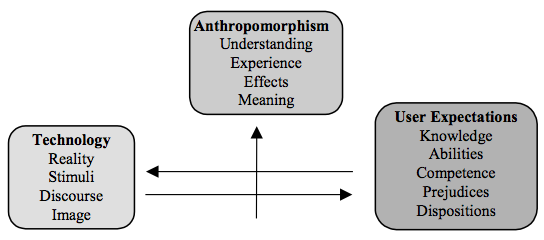
\includegraphics[scale=0.42]{persson_anthropomorphism.png}
% figure caption is below the figure
 \caption{Anthropomorphism emerges in the (real or imagined) interaction between
 robot and user; illustration taken from \cite{persson_anthropomorphism_2000}
 \hl{maybe we don't put the figure here, it was just to illustrate what I mean}}

 \label{fig:anthropomorphism_and_interaction}       % Give a unique label
 \end{figure}

We would like to take up the proposition to discriminate different levels of
anthropomorphism, since each has its own characteristics and involves specific
types of user expectations. This differentiation could allow to draw inferences
on the human-robot relationship from the observed level of anthropomorphism.



\subsection*{A Model of the Dynamics of Anthropomorphism}
\label{sec:dynamics-model}

\paragraph{Why is anthropomorphism likely to change over time?}
\hl{maybe we need to move this paragraph to PART 3}

Why do we think that anthropomorphic projections are likely to change over time
and with growing experience a person has with a robot? The underlying process in
anthropomorphism is understood as reasoning about and perceiving something
non-human, and unknown or unfamiliar based on one's representation of the
familiar and well-known concept of being human (or one-self). The basic
operations underlying inductive inference are the acquisition of knowledge, the
activation or elicitation of knowledge, and the application of activated
knowledge at the time of the judgment \cite{epley_when_2008}. According to Epley
\textit{et al.}, the application includes attempts to correct, adjust, or
integrate less accessible information into a more automatically activated
default representation. This process can be seen as a process of correction, and
thus, it is often insufficient leaving final judgments biased in the direction
of the initially activated representation. As a person's knowledge base changes
/ evolves constantly with newly acquired things, or growing experiences with a
robot, etc., it is likely that the "need to anthropomorphize" a robot decreases
over time. First, because of the evolved knowledge about it, and second because
one has familiarized oneself with it. Consequently, the robot should become more
predictable and more familiar to the human user and inferences about it can be
made based on the acquired knowledge.  /fxfatal{confusing paragraph...needs
reformulation. Could also be turned into a section introduction instead of a
subsection}


So far, the HRI community has not much investigated how anthropomorphism in
human-robot interactions evolves over time (during the process of
\emph{adopting} a robot, for instance): we propose to go beyond the traditional
perception of anthropomorphism in robotics as a static feature that once
observed during a short-term interaction reflects a sustaining social effect.
Based on an extensive literature review previously
published~\cite{fink_anthropomorphism_2012} and field
experiements~\fixme{cites!}, we believe that anthropomorphic effects in HRI are
not always the same but evolve over time, along with growing interaction and
experience with the robot, similar to how relationships among people evolve
over time \fixme{(cite Hinde, 1988)}. In fact, Kanda \textit{et al.}
\cite{kanda_interactive_2004} also hypothesized that people's attitude toward
technological artifacts and their relationship with them would evolve over
time, and they were among the first who described \textit{novelty effects}
during a long-term study with an interactive robot in a school.

The phenomenological model of anthropomorphism we propose
(Figure~\ref{fig:dynamics},~\cite{lemaignan2014dynamics}) represents how the
level of anthropomorphic effects (\ie observable manifestations of
anthropomorphism, as defined in section~\ref{sec:intro}) evolves over a
long-term human-robot interaction. By long-term interaction, we mean direct
(non-mediated), repeated interaction with the same robot, over a long period of
time. 

In this model, anthropomorphism is quantified by a \emph{normalized level of
anthropomorphic effects}: because anthropomorphic effects are not quantified on
an absolute scale, we present them as a normalized value, that spans from a
minimum (no anthropomorphic effects) to a maximum (corresponding to the novelty
effect peak on Figure~\ref{fig:dynamics}). The actual maximum value of
anthropomorphic effects depends on each unique combination of human, robot and
several other factors we introduce below, and thus varies. The general
\emph{shape} of the model remains however the same and depicts the evolution of
anthropomorphism over time, \ie the general dynamics of anthropomorphism.

The model takes into account the duration of the interaction, the nature of the
interaction, as well as acquired experience and familiarization mechanisms. We
also formally introduce a so-called \emph{novelty effect} that models the first
phase of human-robot interaction, during which a specific increase of
anthropomorphic interactions is observed. We focus on \emph{long-term
interaction}, \ie direct (non-mediated), repeated interaction with the same
robot, over an extended period of time (typically longer than a week). The nature 
of the interaction (goal-directed, entertainment, etc.) may
however vary.


\begin{figure*}[htb]
\centering


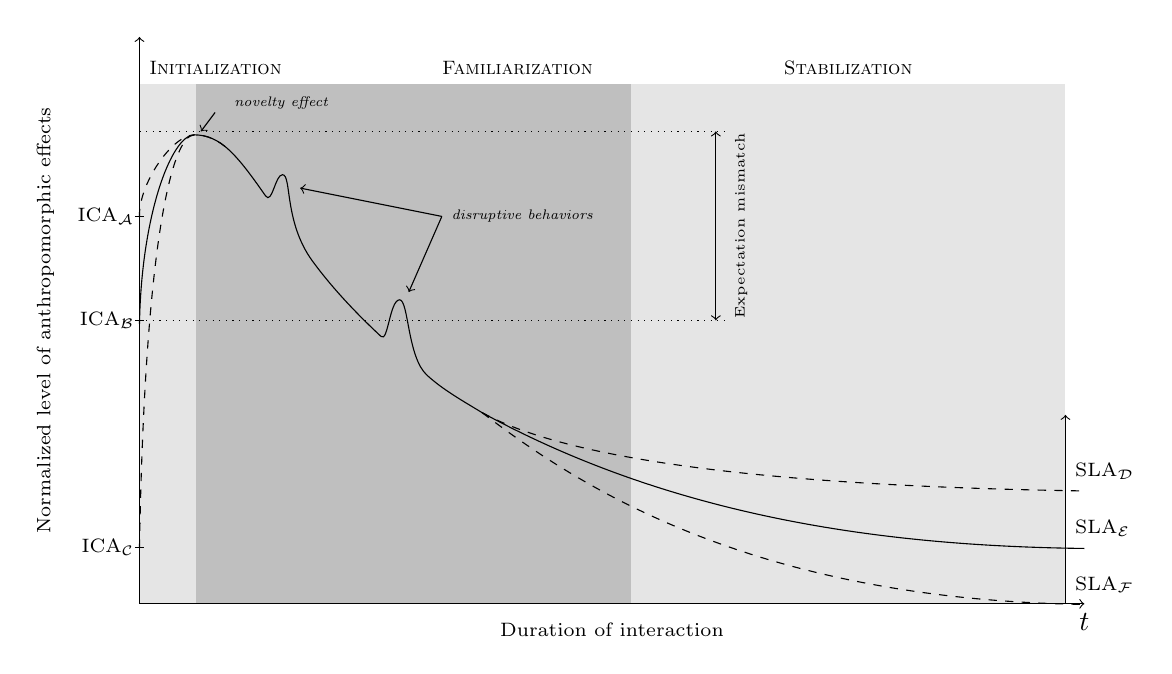
\begin{tikzpicture}[scale=1.2]

% background shading
\path[fill=gray!20] (0,0) rectangle (0.6,5.5);
\path[fill=gray!50] (0.6,0) rectangle (5.2,5.5);
\path[fill=gray!20] (5.2,0) rectangle (9.8,5.5);
\draw(0,5.5) node[anchor=south west] {\scriptsize \sc Initialization};
\draw(4,5.5) node[anchor=south] {\scriptsize \sc Familiarization};
\draw(7.5,5.5) node[anchor=south] {\scriptsize \sc Stabilization};
% horizontal axis
\draw[->] (0,0) -- (10,0) node[anchor=north] {$t$};
\draw(5,-0.1) node[anchor=north] {\scriptsize Duration of interaction};


% vertical axis
\draw[->] (0,0) -- (0,6) node[anchor=east] {};
\draw(-0.8,3) node[rotate=90,anchor=south] {\scriptsize Normalized level of anthropomorphic effects};

\draw (-0.05, 3) -- (0.05, 3) node[anchor=east] {\scriptsize ICA$_{\mathcal B}$};
\draw (-0.05, 4.1) -- (0.05, 4.1) node[anchor=east] {\scriptsize ICA$_{\mathcal A}$};
\draw (-0.05, 0.6) -- (0.05, 0.6) node[anchor=east] {\scriptsize ICA$_{\mathcal C}$};

% vertical axis - end
\draw[->] (9.8,0) -- (9.8,2) node[anchor=east] {};
\draw (9.8, 0.8) node[anchor=west] {\scriptsize SLA$_\mathcal{E}$};
\draw (9.8, 1.4) node[anchor=west] {\scriptsize SLA$_\mathcal{D}$};
\draw (9.8, .2) node[anchor=west] {\scriptsize SLA$_\mathcal{F}$};


\draw[<-] (0.65,5) -- (0.8,5.2) node[anchor=east] {};
\draw (0.9,5.3) node[anchor=west] {\tiny \it novelty effect};


\draw[dotted] (0, 5) -- (6.2,5);
\draw[dotted] (0, 3) -- (6.2,3);
\draw[<->] (6.1,3) -- (6.1,5) node[anchor=east] {};
\draw (6.2,4) node[rotate=90, anchor=north] {\tiny Expectation mismatch};

\draw[<-] (1.7,4.4) -- (3.2,4.1) node[anchor=east] {};
\draw[<-] (2.85,3.3) -- (3.2,4.1) node[anchor=east] {};
\draw (3.2,4.1) node[anchor=west] {\tiny \it disruptive behaviors};
%%%%%
%% CURVES
%%%%
\begin{scope}[yscale=-1,shift={(-0.125,-0.4)}]

% output of inkscape2tikz
\path[draw=black]
    (0.1250,-2.5620) .. controls (0.1451,-3.7193) and (0.4645,-4.5602) ..
    (0.7044,-4.5633) .. controls (0.8413,-4.5633) and (0.9599,-4.5104) ..
    (1.0794,-4.3971) .. controls (1.1989,-4.2841) and (1.3191,-4.1185) ..
    (1.4588,-3.9181) .. controls (1.5287,-3.8183) and (1.5610,-4.1413) ..
    (1.6381,-4.1420) .. controls (1.7378,-4.1420) and (1.6515,-3.6434) ..
    (1.9554,-3.2280) .. controls (2.1466,-2.9667) and (2.3889,-2.7023) ..
    (2.6819,-2.4292) .. controls (2.7551,-2.3607) and (2.7727,-2.8119) ..
    (2.8771,-2.8180) .. controls (2.9742,-2.8180) and (2.9594,-2.2108) ..
    (3.1665,-2.0209) .. controls (3.3340,-1.8673) and (3.5379,-1.7527) ..
    (3.7508,-1.6236) .. controls (5.8366,-0.4852) and (8.0977,-0.2106) ..
    (10.1250,-0.1860);
\path[draw=black, dashed]
    (0.1250,-3.6924) .. controls (0.1103,-4.0298) and (0.4645,-4.5602) .. 
    (0.7044,-4.5633)
    (3.7508,-1.6236) .. controls (4.9579,-0.9555) and (8.1358,-0.8261) .. 
    (10.1250,-0.7946);
\path[draw=black,dashed]
    (0.1250,-0.1953) .. controls (0.1804,-3.3871) and (0.4645,-4.5602) .. 
    (0.7044,-4.5633) .. controls (0.8413,-4.5633) and (0.9599,-4.5104) .. 
    (1.0794,-4.3971)
    (3.7508,-1.6236) .. controls (4.7654,-0.8505) and (6.5955,0.3538) .. 
    (10.1250,0.4062);

\end{scope}

\end{tikzpicture}

\caption{The dynamics of anthropomorphism. We distinguish three main phases:
    \emph{initialization}, \emph{familiarization} and \emph{stabilization},
    preceded by a \emph{pre-interaction} phase. In the pre-interaction phase,
    users build an \emph{initial capital of anthropomorphism} (ICA). Once the
    interaction starts, the level of anthropomorphism increases due to the
    \emph{novelty effect}~\cite{kanda_interactive_2004}, and then decreases to
    reach a \emph{stabilized level of anthropomorphism} (SLA).  During the
    interaction, unpredicted behaviors of the robot (\emph{disruptive behaviors})
    may lead to local increase of the level of anthropomorphism.}

\label{fig:dynamics}
\end{figure*}

\subsection*{Three phases}
\label{sec:phases}

We distinguish three main phases that describe the evolution of the
anthropomorphic effects in a long-term human-robot interaction. They are
depicted in different shades on Figure~\ref{fig:dynamics}.

First, the \emph{initialization} phase. During this short phase (from a couple
of seconds to a couple of hours), we observe an increased level of
anthropomorphism, from an \emph{initial capital of anthropomorphism}
(detailed in the next section) to a peak of anthropomorphic manifestations
that corresponds to the maximum of the \emph{novelty effect}.
Section~\ref{sec:initialization} details this first phase.

The second phase, \emph{familiarization}, lasts longer (up to several days) and
models the process of the human getting acquainted to the robot: by observation
and interaction, the human builds a model of the robot's behavior that allows
him/her to predict the robot's actions. We observe a decrease of
anthropomorphic effects during this phase, that we explain by the acquired
ability to predict the behavior of the robot: the initial apparent behavioral
complexity vanishes, and the robot is considered more and more as a tool.
Section~\ref{sec:familiarization} discusses the second phase.

The last phase is the \emph{stabilization} phase. The level of anthropomorphic
effects tends to stabilize over a longer time, to reach a \emph{stabilized
level of anthropomorphism} (SLA). The SLA may be null (no anthropomorphic
effects observed anymore), but it may also remain at a higher level.  This
third phase, as well as the \emph{stabilized level of anthropomorphism}, are
discussed in section~\ref{sec:stabilization} below.

\subsection*{Initialization Phase}
\label{sec:initialization}

\paragraph{Initial Capital of Anthropomorphism}
\label{sec:ica}

The \emph{initial capital of anthropomorphism} describes the initial potential
for the robot to be anthropomorphized by the human user in a given situation.
This potential depends on several factors. It has been shown, for instance, that
some \textit{people} tend to anthropomorphize more than others, that some
\textit{situations} induce anthropomorphism more than others, that
\textit{children} tend to anthropomorphize more than adults, and that some
\textit{cultures} are notorious for their anthropomorphic religions and
worldviews~\cite{epley_when_2008}. Also the shape and design of the robot play a
role, and the context in which the interaction takes place. Our model of
anthropomorphism takes these determinants into account and initializes the level
of anthropomorphic interactions between a human and a robot to a value that we
call \emph{initial capital of anthropomorphism} (ICA). The ICA describes the
first (real or imagined) contact to a robot. In this stage of pre-interaction,
people form initial expectations toward the robot and imagine how they will use
it / interact with it.

We build the ICA on three main factors that \emph{a priori} determine the
potential that a robot will be anthropomorphized:

\begin{enumerate}

    \item \emph{Human-centered factor}: The \textbf{personality} and individual
        traits of the human user: Psychological characteristics / determinants
        that influence a person's tendency to anthropomorphize
        artifacts~\cite{epley_seeing_2007}. Other individual traits and
        demographic aspects are comprised (\eg age, gender, cultural background,
        professional background).

    \item \emph{Robot-centered factor}: The robot's \textbf{design} and how it
        appears to the human user. Characteristics of the robot's form,
        behavior, and interaction modalities (anthropomorphic
        design)~\cite{fong_survey_2003}.

    \item \emph{Situation-centered factor}: The real or imagined
        \textbf{purpose} of the robot, including the situational context in
        which it is used, as well as the task context and role in which the
        robot is used / experienced (environmental
        context)~\cite{joosse_what_2013}.

\end{enumerate}	

The ICA comprises some hypothetical values for each of these three factors, such
that different ICA values can be obtained, given the robot, human user, and
environmental context\fxfatal{??}.

For \textbf{personality}, we suggest to apply Epley \textit{et al.}'s
\cite{epley_seeing_2007} psychological \textit{"Three Factor Theory"} of
anthropomorphism. For instance, children generally tend to anthropomorphize
objects more than adults. Also, a person who lacks social connection is said to
be more likely to anthropomorphize. Both aspects would increase the ICA. This
means that, one and the same robot used by a different user, can lead to a
different ICA.

For \textbf{design}, we understand that a robot that follows an anthropomorphic
design (\eg NAO) leads to a higher ICA than a rather functional robot (\eg
Roomba). Also, a robot that is able to display facial expressions would increase
the ICA. However, \hl{as discussed before} a classification of the "amount" of
anthropomorphic design in a robot, as for instance suggested by Fong \textit{et
al.} \cite{fong_survey_2003}, can be difficult. Nevertheless, the important
aspect is how the robot appears to the user, \eg human-like or machine-like.
Studies have shown that an anthropomorphic robot is perceived differently to a
non-anthropomorphic robot\fxfatal{...this sentence sounds strange like that.
Need references or better integration in the paragraph}.

By taking the \textbf{purpose} of a robot into account, we suggest that the real
or imagined context in which a robot is used and the interaction that this usage
brings along, impacts how far the robot will be attributed human-like
characteristics. We draw on findings such as presented in Joosse
\etal~\cite{joosse_what_2013}. The authors showed for instance that when the
same robot (NAO) is used in a different task context (cleaning task \emph{vs.}
tour guide), users ascribe different ``personalities'' to the robot. In general,
a robot which is imagined to be used in a social, entertaining or playful
context leads to a higher ICA than a robot which is used for a routine or
focused task (security, rescue, etc.). This idea also receives support from
Goetz \& Kiesler's work that revealed that people prefer a serious robot for
serious tasks and a less serious robot for more playful
tasks~\cite{goetz_cooperation_2002, goetz_matching_2003}. Also, we suggest that
the environmental context in which people experience and interact with the robot
impacts the ICA. For instance, several friends interacting simultaneously with
the robot might lead to increased ICAs, due to increased human-human social
interactions (the robot might be perceived to be part of the social interaction,
and in turn attributed human-like qualities)~\cite{baxter2013do}.

\paragraph{The Novelty Effect}
\label{sec:noveltyeffect}

TDB

\subsection*{Familiarization Phase}
\label{sec:familiarization}

\emph{Familiarization}, in this context, means \emph{to get acquainted with}.
It is not to be confused with the \emph{familiarity thesis} that relates to the
projection of already known cognitive models onto the robot. We discuss this other
aspect at section~\ref{sec:cognitivemodel}.

The \emph{familiarization phase} starts at the peak of the \emph{novelty
effect}: anthropomorphic effects are at their maximum, the user thinks (s)he is
potentially facing an agent aiming at ``human-level intelligence'' (to take
McCarthy's words). This is a transient state that quickly vanishes, and the
projected anthropomorphism then starts to decrease while the human observes and
recognizes that the behaviour of the robot is generally \emph{predictable} and
possibly \emph{deceptive} (for instance, it talks but does not understand when
we talk ; it has eyes but does not recognize everyday objects we show ; etc.).

\paragraph{Disruptive behaviors}

By \emph{disruptive behaviors}, we mean any behavior exhibited by the robot
that is unexpected by the user: for instance, a robot may usually follow always
the same route to go to two different places in a house, and suddenly change
the route. The actual underlying reason may span from a bug to the detection of
a new possible obstacle, but as long as this reason is not immediately
intelligible to the user, the behavior counts as \emph{disruptive}.

Our model represents \emph{disruptive behaviors} as local increases of
anthropomorphic effects in the familiarization phase (and at a lesser extend,
in the stabilization phase) (Figure~\ref{fig:dynamics}): because such behaviors
are unexpected, a human observer may interpret them as the result of a richer
deliberative process, which in turn leads to the supposition of complex
cognitive skills

This is however to be modulated depending on the real and percieved reasons of the
unexpected behavior.  Section~\ref{sec:disruptive} discusses more in depth the
mental correlates of disruptive behaviors. It proposes a typology that relates
them to the anthropomorphism they induce. It may increase if the user perceives
(rightfully or not) a form of intentionality, as well as decrease if the
unexpected behavior is perceived as a failure.

\paragraph{Expectation mismatch}

Besides, we propose to call \emph{expectation mismatch} the delta between the
initial capital of anthropomorphism for a given tuple (user, robot, context)
and the anthropomorphism peak of novelty effect (Figure~\ref{fig:dynamics}).
\fixme{Need to rediscuss what this delta actually represent...}

\subsection*{Stabilization Phase}
\label{sec:stabilization}

The last phase is the \emph{stabilization} phase. The level of anthropomorphic
effects tends to stabilize over a longer time, to reach a \emph{stabilized
level of anthropomorphism} (SLA).

If, after the familiarization phase, no anthropomorphic effects are observed
anymore, the \emph{Stabilized Level of Anthropomorphism} is zero. This can
be interpreted as the user interacting with the robot in a routine way, without
projecting anymore human-like traits on the robot.


\paragraph{Stabilized Level of Anthropomorphism (SLA)}

The \emph{Stabilized Level of Anthropomorphism} (SLA on
Figure~\ref{fig:dynamics}) describes the long-term lasting level of
anthropomorphism.  Like the ICA, the SLA has a unique value per triplet
(\emph{human}, \emph{robot}, \emph{context of interaction}).

We proposed that the ICA is built on three factors: user's \emph{personality},
robot's \emph{design} and interaction \emph{purpose} (or \emph{interaction
context}). The user's personality and the context of use do also influence the
SLA. In particular, it appears that the user's level of acquaintance with
technologies plays an important role in long-term tendency to
anthropomophize~\cite{fink_living_2013} (people more familiar with technology
understand, and hence predict, better the behavior of the robot, which in turn
leads them more frequently to ultimately consider the robot as a simple tool).

The robot's design, on the other hand, plays a more subtle role, and strong
initial anthropomorphic design does not mandate high SLA: lasting
anthropomorphic effects have been observed on non-anthropomorphic robots (like
the iRobot Roomba~\cite{fink_living_2013} or the military iRobot
PackBot\footnote{Rodney Brooks has reported in keynotes that occasionally
soldiers would give a name to \emph{their} PackBot and require it to be repaired
instead of being replaced by another one in case of incident.}), and on the
contrary, anthropomorphic designs can lead to higher expectation deceptions,
resulting in the robot not being used anymore.

Note that the \emph{Initial Capital of Anthropomorphism} and the
\emph{Stabilized Level of Anthropomorphism} are generally not correlated: one
individual may have high potential of anthropomorphizing (high ICA) at first
sight of a good-looking humanoid robot, and get disappointed by the actual
abilities of the robots, down to routine, non-anthropomorphic, interactions (low
SLA), while another user with the same high ICA may, for instance, creates
lasting affective bonds with the same robot, and keeps anthropomorphizing it
(higher SLA).



%%%%%%%%%%%%%%%%%%%%%%%%%%%%%%%%%%%%%%%%%%%%%%%%%%%%%%%%%%%%%%%%%%%%%%%%%
%
%
%
%		PART 3: EXPLANATIONS -- COGNITIVE CORRELATES, NEUROSCIENCE VIEW
%
%
%
%%%%%%%%%%%%%%%%%%%%%%%%%%%%%%%%%%%%%%%%%%%%%%%%%%%%%%%%%%%%%%%%%%%%%%%%%
%
% CLAIRE & SEVERIN:
%
%

\vspace{2cm}
\section{Cognitive Correlates and Neuroscience Perspective}
\label{sec:cognition-neuroscience}

In this section, we discuss more speculative aspects and hypotheses that follow
from the model. These aspects would benefit further investigations and
experimental support.

\subsection*{Cognitive Interpretations}
\label{sec:cognitive-model}


\begin{figure}[htb]
\centering
%\resizebox{\linewidth}{!}{
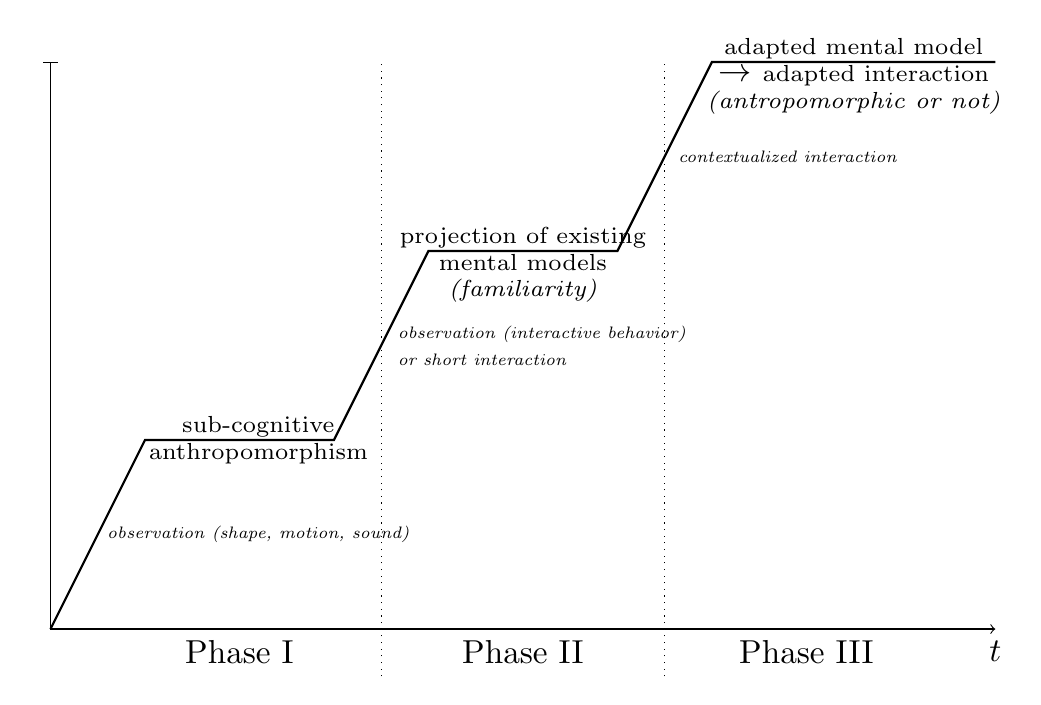
\begin{tikzpicture}[scale=1.2, transform shape]
\baselineskip=8pt

% horizontal axis
\draw[->] (0,0) -- (10,0) node[anchor=north] {$t$};
% labels
\draw   (2,0) node[anchor=north] {Phase I}
        (5,0) node[anchor=north] {Phase II}
        (8,0) node[anchor=north] {Phase III};

\draw[dotted] (3.5, -0.5) -- (3.5,6);
\draw[dotted] (6.5, -0.5) -- (6.5,6);

% vertical axis
\draw[-|] (0,0) -- (0,6) node[anchor=east] {};
% Us
\draw[thick] (0,0) -- (1,2) -- (3,2) -- (4,4) -- (6,4) -- (7,6) -- (10,6);

\draw (2.2,2) node[align=center] {\scriptsize{sub-cognitive}\\\scriptsize{anthropomorphism}}; %label
\draw (5,3.85) node[align=center] {\scriptsize{projection of existing}\\\scriptsize{mental models}\\\scriptsize{\it (familiarity)}}; %label
\draw (8.5,5.85) node[align=center] {\scriptsize{adapted mental model} \\ $\to$ \scriptsize{adapted interaction}\\\scriptsize{\it (antropomorphic or not)}}; %label

\draw (2.2,1) node[align=left] {\tiny{\it observation (shape, motion, sound)}}; %label
\draw (5.2,3) node[align=left] {\tiny \it observation (interactive behavior) \\ \tiny \it or short interaction}; %label
\draw (7.8,5) node[align=left] {\tiny \it contextualized interaction}; %label

\end{tikzpicture}
%}
\caption{The three cognitive phases of anthropomorphism: Phase I is the instinctive,
sub-cognitive identification of living peers. {\it Empathy} is characteristic
of this stage. After longer observation or short, non-contextualized interaction
(typically, a lab environment), the user enters Phase II: the user projects a
mental model he/she is already familiar with onto the robot. After longer {\it
contextualized} interaction (typically, at home), the user enters Phase III of
anthropomorphism: the user recomposes an accurate mental model of the robot,
based on experience. This leads to adapted interaction modalities, that may
still be anthropomorphic, or not.}
\label{fig:cognitivemodel}
\end{figure}


We provide in this section a tentative interpretation of anthropomorphism in
terms of cognitive correlates. We warmly welcome the feedback and
comments from both the cognitive sciences and robotics communities to further
discuss these findings.

We propose three different cognitive phases (Figure~\ref{fig:cognitivemodel}),
which do not directly match the previously presented three phases of
anthropomorphism but are still related.


\subsection*{Cognitive Processes and Phases}

The main underlying cognitive process in anthropomorphism is understood as
perceiving and reasoning about something non-human and unfamiliar based on one's
representation of the familiar and well-known concept of being
human~\cite{epley_when_2008}. This led us to interpret the phases of
anthropomorphic interactions as parallel cognitive phases
(Figure~\ref{fig:cognitivemodel}).

The so-called \emph{phase I} is the instinctive, pre-cognitive identification of
living peers. That humans tend to anthropomorphize robots intuitively in this
pre-cognitive way
is supported by studies done by Rosenthal-von der Pütten
\textit{et al.}~\cite{rosenthal-vonderputten_experimental_2013} who investigated
the neural correlates of emotional reactions of humans towards a robot. {\it
Empathy} is characteristic of this stage~\cite{rosenthalvonderPutten2013neural}.
Anthropomorphism at this pre-cognitive stage might also be mediated by the
human's mirror neurons system (neurons that fire both during execution of
specific goal-oriented action and during the viewing of action directed toward
the same goal~\cite{Rizzolatti1996, Kilner2009}) by allowing for a mapping of
the robot's goal-directed actions into the human own motor
repertoire~\cite{Gallese1998, Wolpert2003, cullen2013individual}.

After a longer observation period (typically including complete action sequences
of the robot) or short interaction (touching, short talk like greetings), we
suggest the human enters the cognitive \emph{phase II}: in this phase, the human
starts building a behavioral and cognitive model of the robot that would support
both the observed and imagined capabilities of the robot.  The \emph{familiarity
thesis}~\cite{hegel_understanding_2008} supports the idea that the human
first projects onto the robot mental models of similar agents he/she is already
familiar with (ranging from animals to human adults, to pets and children). We 
hypothesize that the nature of the projected mental
model, as well as how deep the human engages in this projection, might be
driven by the same parameters as we mentioned for the \emph{initial capital of
anthropomorphism} (section~\ref{sec:ica}).

The cognitive \emph{phase III} occurs after a \emph{contextualized} interaction.
A \emph{contextualized} interaction is \emph{explicitly purposeful} (the purpose
of the interaction, be it purely entertainment, is explicit and conscious to the
human), and takes place in an environment that fosters a stronger cognitive (and
possibly affective/social) commitment from the human in the interaction
(typically, at home). During this interaction, the human iteratively restates
and reshapes his/her behavioral and mental model of the robot (\emph{How does
the robot react to such and such situation/input?  What does the robot know
about me? About itself? About our environment? What can the robot learn?}, etc.).

This mental process depends on the human understanding of the robot's
inner working, as well as his/her own tendency to anthropomorphize (the
\emph{personality} in ICA factor), but at this
stage, the \emph{perception} of the robot (its shape for instance) and its
intended \emph{purpose} play a less important role. It is mostly a human-centric
process.  The result of this third phase would be an iteratively adapted
cognitive model of the robot.


\subsection*{Relation to the model of anthropomorphism}

These cognitive phases overlap but do not exactly match the
\emph{Initialization}, \emph{Familiarization} and \emph{Stabilization} phases
introduced in our model of the dynamics of anthropomorphism. In particular,
cognitive phases I and II are both included in the \emph{initialization} phase
of the anthropomorphism model. Sub-cognitive anthropomorphism typically
\emph{initiates} the novelty effect by rapidly engaging the human in the
interaction through an initial projected agency, whereas cognitive phase II
(projection of familiar mental models) supports the novelty effect by inducing
beliefs that the robot is set up with possibly complex cognitive abilities.

The cognitive phase III also overlaps with the \emph{familiarization} phase: as
the human gets used to the robot, we hypothesize one restates and adapts its
cognitive model of the robot by iteratively reshaping pre-existent, familiar
models until it provides a satisfying support to explain and justify the
observed robot behavior.

A \emph{stable level of anthropomorphism} is reached when the adaptation process
depicted in cognitive phase III reached a stable state, \ie the user's
experience with the robot is correctly supported by the cognitive model he/she
has built.

\paragraph{Limits} This discussion on the cognitive correlates of the dynamics
of anthropomorphism are speculative, and only indirectly supported by
experimental evidence. New experiences need to be designed to specifically test
these hypothesis.\fxnote{...}


\begin{itemize}
    \item \textbf{Hypothesis 1} A person's tendency to anthropomorphize a robot
        is impacted by the context of use and purpose of the robot. A social
        context and purpose of the robot increases anthropomorphism.
        \textit{(context and purpose of the robot)}
	\item \textbf{Hypothesis 2} A person's tendency to anthropomorphize a robot decreases over time and with growing experience the person has with the robot. \textit{(familiarize oneself with the robot)}
\end{itemize}

\subsection*{Impact of the behavioral complexity of robots}

TBD. Most experiments are carried with robots exhibiting relatively simple
behaviors. In our model, the maximum level of anthropomorphism is reached with
the novelty effect, and then decrease. Can we go \emph{over} the novelty effect
if the robot exhibit more complex behaviors?

\subsection*{Segmentation of interaction phases}

TBD

\subsection*{Behavioral cues of anthropomorphism}
\label{sec:behavioralcues}

Our model suggests to analyze anthropomorphism based on a \emph{relative and
normalized level of anthropomorphic effects} instead of an absolute
quantitative assessment of anthropomorphic evidences. Similarly we introduce
two specific \emph{abstract} levels of anthropomorphism, the \emph{Initial
Capital of Anthropomorphism} and the \emph{Stabilized Level of
Anthropomorphism}: while we discuss the factors on which those values are
build, we did not formally investigated the experimental cues or evidences
that would allow to actually quantify those levels.

The intricacy and interdependency of those behaviors make them difficult to
quantify.  Their systematic identification and interpretation rely on
psychosomatic cues that the authors did not investigate.

A formal methodology for the assessment of anthropomorphic effects in HRI, as
well as a typology of these effects is still to be formally devised.

\subsection*{Effect of Time and Familiarization}

The \textit{context of use} is related to the purpose (and functionality) of the
robot and influences the user interaction experience. With \textit{time}, we
refer to long-term interaction with the robot, which is related to what has been
described as \textit{novelty effect} but also accounts for the user getting used
to the robot. Consequently, we propose that anthropomorphism is not static but
likely to change, due to what we call \textit{dynamics}, in space and time.


As outlined in section \hl{XX}, the tendency to anthropomorphize is motivated by
a person's wish to make sense of an agent which might be difficult to understand
(in its functionality or behavior, for instance). In turn, a user might ascribe
intentions or emotions to the system because the systems output was unexpected
for the user. Based on this explanation, we estimate that when the user has
familiarized herself / himself with the system, thus reached the point of when
the system is usable and explainable, the tendency to anthropomorphize
decreases. Therefore, our second hypothesis is as follows: 

\begin{itemize}
	\item \textbf{Hypothesis 2} A person's tendency to anthropomorphize a robot decreases over time and with growing experience the person has with the robot. \textit{(familiarize oneself with the robot)}
\end{itemize}	
	

Given our first hypothesis from above, this might not hold over all contexts;
more concretely, probably not in a social context of usage.


Smart innovative devices, such as personal domestic robots, might demand from a
human user spontaneous usage of an unfamiliar system. Such situations will
require that a user should be able to build up a mental model quickly, which
particularly holds for novice users \cite{schmitz_concepts_2011}.

Eddy \textit{et al.} points out that familiarity increases the tendency to
anthropomorphize \cite{eddy_attribution_1993}.

"As shown in several psychological experiments [13,24] and pointed out by Watt
[25], familiarity may also ease social acceptance and even tend to increase
people's tendency to anthropomorphize [16]." \cite{duffy_anthropomorphism_2003}


\subsection*{Role of disruptive behaviors}
\label{sec:disruptive}

Common observation of naive people (children or adults) interacting with robots
shows that unexpected behaviors of the robot can have a notable impact on
interaction. \hl{cite literature, e.g. cheating robot, disagreeing, disobeying,
HRI2013 paper}

During a normal interaction with the robot, the user iteratively refines his/her
own model of the behavior of the robot. As explained in previous sections, as
the user improves his/her model of the robot's actions, he/she also improves the
ability to predict the actions and thus, the user tends to anthropomorphize
less.

We emit the hypothesis that an unexpected robot behavior might lead the user to
suddenly restate his/her behavioral model of the robot and will temporarily lead
to an increase of the level of anthropomorphism (depicted by the spikes on
Figure~\ref{fig:dynamics}).



\begin{figure}\footnotesize
    \begin{tabular}{  >{\centering\arraybackslash}m{2cm} | >{\centering\arraybackslash}m{2cm} | >{\centering\arraybackslash}m{2cm} }
     & Unplanned by the robot & Planned by the robot \\ \hline
    Perceived as non-intentional & case I  & case IIIa  \\ \hline
    Perceived as intentional &  case IIIb & case II 
    \end{tabular}
\caption{
    Behaviors of the robot that are unexpected by the user may be intentional
    (the robot has planned the behavior) or not (typically, a failure:
    misdetection, bug,...). Independently of that, the behavior may be
    \emph{perceived} by the user as intentional or not.}
\label{fig:perceptionUnexpectedBehavior}
\end{figure}

When talking about \emph{unexpected robot behaviors}, several distinct cases
must however be considered, summarized in
Table~\ref{fig:perceptionUnexpectedBehavior}.

If the unexpected behavior is not planned, and perceived as such by the human
(case I), the human can interpret that the robot is able to fail. If the robot
explicitly states its failure (for instance, by saying ``I'm lost!''), the
behavior is then called \emph{transparent} \fixme{cite here, Julia?}
\hl{(literature on transparency)}, and the user may besides hypothesize that the
robot has \emph{introspective} capabilities (it can reflect on its own internal
state), which in turn may leads to higher anthropomorphism level.  On the
contrary, if the robot shows no sign of recognizing its own failure, the user
may ascribe a lower level of anthropomorphism to the robot.

In case II, the robot voluntary executes a behavior that is unexpected by the
human, and the human perceives it rightfully as an \emph{intentional} behavior.
For instance, the human asks the robot to go somewhere, and the robot refuses,
saying ``I do not want to go there''. In that case, we expect to see an increase
of anthropomorphism attribution due to the human ascribing intentionality to the
robot.

Case IIIa and IIIb correspond to misinterpretations of the robot behavior. Case
IIIb may actually lead to an increased level of anthropomorphism since the human
will (wrongfully) attribute intentionality to the robot, while case IIIa is
expected to lead to a lower anthropomorphism level.  However, in those two
cases, the next occurrence of an expected behavior, if correctly interpreted
(case I or II), is likely to lead to stronger effects due to a larger delta
between expectations and actual observed behavior. \hl{(we actually assume that
anthropomorphism can be radically changing and be a very spontaneous
"reaction".)}

%% experience -> unexpected behavior should not impact the interaction child-robot BEFORE the theory of mind is established!


%%%%%%%%%%%%%%%%%%%%%%%%%%%%%%%%%%%%%%%%%%%%%%%%%%%%%%%%%%%%%%%%%%%%%%%%%
%
%
%
%				DISCUSSION + FUTURE WORK
%
%
%
%%%%%%%%%%%%%%%%%%%%%%%%%%%%%%%%%%%%%%%%%%%%%%%%%%%%%%%%%%%%%%%%%%%%%%%%%

% JULIA & SEVERIN: how to measure / quantify anthropomorphism ...
% CLAIRE: FMRI study idea

\vspace{2cm}
\section{Discussion}
\label{sec:discussion}

The model of anthropomorphism we propose is still a work in progress. In
particular, its implications regarding the design of (social) robots and
human-robot interaction are still to be refined.

This interpretation of anthropomorphism in terms of cognitive correlates opens
questions that we hope could be fruitfully discussed during the workshop.  By
adopting both a cognitive and a dynamic perspective on the anthropomorphic bonds
that establish between a robot and a human during an interaction, some
observations can be raised.

For instance, we propose that the human \emph{adapts} iteratively to the robot
by restating its cognitive model of the robot. Could our two models be
conversely relied on to have the robot itself iteratively adapting its
behaviour? In particular, we hypothesize that the so-called novelty effect
represents a peak in anthropomorphic manifestations, followed by mostly
deception-driven refinements of the cognitive behavioural model of the robot.
Could we imagine that the robot pro-actively \emph{verbalises} its own limits,
in a timely manner (likely before the end of the novely effect). And how would
this affect the cognitive models built by the human?

One related question we plan to elaborate on is the effects of \emph{mutual
explicitation of the mental model of the other agent}: a human and a robot
interact on a given task, and after a while, we interrupt the task and ask each
of the agents to explicit the mental model it has built of its partner
(emotional state, beliefs, intentions, etc.). Depending on the cognitive phase
the two agents are in, we may expect varying accuracy levels in the produced
mental models.

Another question raised by these models relates to their transposition to
human-human interaction: while concepts like \emph{novelty effect} are not
directly meaningful when analyzing human-human interaction, insights from
cognitive sciences (and in particular social psychology) regarding how we, as
humans, cope with unexpected behaviours from peers, or on the dynamics of mental
model refinements, could bring interesting perspectives with possible
applications to better manage long-term human-robot interactions.

%%%%%%%%%%%%%%%%%%%%%%%%%%%%%%%%%%%%%%%%%%%%%%%%%%%%%%%%%%%%%%%%%%%%%%%%%
%
%
%
%				CONCLUSIONS
%
%
%
%%%%%%%%%%%%%%%%%%%%%%%%%%%%%%%%%%%%%%%%%%%%%%%%%%%%%%%%%%%%%%%%%%%%%%%%%

% JULIA & SEVERIN

\vspace{2cm}
\section{Conclusion}
\label{sec:conclusion}

Anthropomorphism is a social phenomenon which seems to be natural on one side
and very complex on the other side. It is a mechanism within oneself that makes
a human observer think and treat a non-human agent as if it would have some
human (social) characteristics, and ascribe to it intentions, emotions, or
thoughts, for instance. Understanding the reasons and modalities of
anthropomorphism is thus of prime importance to build a successful and lasting
human-robot interaction.

While anthropomorphism is traditionally empirically understood as the
interactions between the anthropomorphic design of a robot and the psychological
determinants of the user, it appears that the duration and context of the
interaction are also key factors, and that anthropomorphism needs to be
understood as a dynamic phenomenon. In this article, we propose a new formal
model of anthropomorphism that accounts for these three factors and also
explicits the dynamics of anthropomorphism. We introduce the concepts of
\emph{initial} and \emph{stabilized levels of anthropomorphism} as compound
factors to characterize the profile of a given anthropomorphic interaction.

The article also discusses the cognitive correlates of anthropomorphism. We
proposes to identify three cognitive phases corresponding to successive
refinements of the mental models of the robot that the user builds during the
interaction. We show how these phases relate to observable anthropomorphic
effects, and how they evolve over time.

While subject to discussion and further extensions, we hope that this
contribution consolidates the scientific grounds of anthropomorphism, and
provides support for a better understanding of long-term acceptance of robots in
human environments.

\vspace{2cm}
\section*{Acknowledgments}

We would like to acknowledge the fruitful discussions with A Jung Moon and
Aude Billard.

This research was supported by the Swiss National Science Foundation through
the National Centre of Competence in Research Robotics.

\vspace{2cm}
\section*{Bibliography}

\bibliographystyle{frontiersinSCNS&ENG} % for Science and Engineering articles
\bibliography{dynamics-anthropomorphism}   % name your BibTeX data base


\end{document}
